\documentclass{article}
\usepackage{graphicx} % Required for inserting images
\usepackage[most]{tcolorbox}
\usepackage{amsmath}
\usepackage{amssymb}
\usepackage{dsfont}
\usepackage{float}
\usepackage{colortbl}
\usepackage[left=2cm,right=2cm,top=2cm]{geometry}

\title{MAA106}
% \author{daniela.cojocaru }

\definecolor{light-green}{rgb}{0.85,0.96,0.84}
\definecolor{dark-green}{rgb}{0.29,0.43,0.27}
\definecolor{dark-blue}{rgb}{0.21,0.32,0.52}
\definecolor{light-blue}{rgb}{0.85, 0.94,0.98}
\definecolor{light-red}{rgb}{0.99,0.94,0.91}
\definecolor{dark-red}{rgb}{0.66,0.05,0.01}
\definecolor{light-yellow}{rgb}{0.97,0.92,0.81}
\definecolor{dark-yellow}{rgb}{0.72,0.43,0.12}

\newtcolorbox{definition}[1]{% 
    enhanced,
    colback=light-green, % Background color
    colframe=black,  % Border color
    %sharp corners,
    rounded corners, %=northeast, % Rounded corners on the top-right
    fonttitle=\bfseries,
    boxsep=2mm,
    top=3mm,
    boxrule=0.5mm,
    overlay={
        \node[
            anchor=north west,
            xshift=-2mm,
            yshift=2mm,
            % boxrule=1mm,
            text=dark-green, 
            fill=white, 
            draw=dark-green,
            rounded corners,
            %inner ysep=2mm, % Added inner padding
            font=\large\bfseries
        ] at (frame.north west) {Definition - #1};
    }
}

\newtcolorbox{remark}{% 
    enhanced,
    colback=light-blue, % Background color
    colframe=black,  % Border color
    %sharp corners,
    rounded corners, %=northeast, % Rounded corners on the top-right
    fonttitle=\bfseries,
    boxsep=2mm,
    top=3mm,
    boxrule=0.5mm,
    overlay={
        \node[
            anchor=north west,
            xshift=-2mm,
            yshift=2mm,
            % boxrule=1mm,
            text=dark-blue, 
            fill=white, 
            draw=dark-blue,
            rounded corners,
            %inner ysep=2mm, % Added inner padding
            font=\large\bfseries
        ] at (frame.north west) {Remark};
    }
}

\newtcolorbox{other}[1]{% 
    enhanced,
    colback=light-red, % Background color
    colframe=black,  % Border color
    %sharp corners,
    rounded corners, %=northeast, % Rounded corners on the top-right
    fonttitle=\bfseries,
    boxsep=2mm,
    top=3mm,
    boxrule=0.5mm,
    overlay={
        \node[
            anchor=north west,
            xshift=-2mm,
            yshift=2mm,
            % boxrule=1mm,
            text=dark-red, 
            fill=white, 
            draw=dark-red,
            rounded corners,
            %inner ysep=2mm, % Added inner padding
            font=\large\bfseries
        ] at (frame.north west) {#1};
    }
}

\newtcolorbox{theorem}[1]{% 
    enhanced,
    colback=light-yellow, % Background color
    colframe=black,  % Border color
    %sharp corners,
    rounded corners, %=northeast, % Rounded corners on the top-right
    fonttitle=\bfseries,
    boxsep=2mm,
    top=3mm,
    boxrule=0.5mm,
    overlay={
        \node[
            anchor=north west,
            xshift=-2mm,
            yshift=2mm,
            % boxrule=1mm,
            text=dark-yellow, 
            fill=white, 
            draw=dark-yellow,
            rounded corners,
            %inner ysep=2mm, % Added inner padding
            font=\large\bfseries
        ] at (frame.north west) {#1};
    }
}

\newtcolorbox{algo}[1]{
    enhanced,
    colback=gray!20, % Background color
    colframe=black,  % Border color
    sharp corners,
    % rounded corners, %=northeast, % Rounded corners on the top-right
    fonttitle=\mdseries,
    fontupper=\ttfamily,
    boxsep=0mm,
    top=5mm,
    boxrule=0.1mm,
    overlay={
        \node[
            anchor=north west,
            xshift=-2mm,
            yshift=2mm,
            % boxrule=1mm,
            text=black, 
            fill=white, 
            draw=black,
            % rounded corners,
            %inner ysep=2mm, % Added inner padding
            font=\large\mdseries
        ] at (frame.north west) {#1};
    }
}

\begin{document}
% \maketitle
\begin{flushright}@usercdp\end{flushright}

\section{Root finding for a function of one variable}

    \subsection{Convergence / order of convergence}

        Let us write the following problems under the generic root-finding form:
        \begin{equation}
            \text{given } f: [a,b] \rightarrow \mathbb{R}, \text{ find } x^* \in [a,b] \text{ such that } f(x^*)=0 \nonumber
        \end{equation}

        % \vspace{0pt}

        \begin{definition}{Convergence}
            Suppose that a sequence $(x_k)_k$ is generated to approximate $x^*$. The error at step $k$ is defined as
            
            \centerline{$e_k = |x_k - x^*|. $}
            

            The sequence $(x_k)_k$ is said to \textit{converge} to $x^*$ if

            \centerline{$e_k \longrightarrow 0$ when $k \rightarrow \inf$}
        \end{definition}

        \vspace{10pt}

        \begin{definition}{Order of convergence for iterative algorithms}
            Suppose that the sequence $(x_k)_k$ converges to $x^*$. We say that its \textit{order of convergence} is $\alpha \geq 1$ if 

            $$\exists C > 0, e_{k+1} \underset{k\to\infty}{\sim} C e_k^\alpha$$

            or equivalently, if
            
            $$
            \exists C>0,  \quad{} \frac{e_{k+1}}{e_k^\alpha} \underset{k\to\infty}{\rightarrow} C.
            $$


            The convergence is said to be
            
            \hspace{20pt}$\bullet$ \textbf{sublinear} if $\alpha=1$ and $C=1$,
            
            \hspace{20pt}$\bullet$ \textbf{linear} if $\alpha=1$ and $C<1$,
            
            \hspace{20pt}$\bullet$ \textbf{quadratic} if $\alpha=2$.
            \vspace{4pt}
            
            The constant $C$ is sometimes called the \textit{rate} of convergence. 
        \end{definition}

        \vspace{10pt}

        \begin{remark}
            $\bullet$ If we have an estimate of the form
            \vspace{4pt}

            \centerline{$\exists C > 0, e_{k+1} \leq C e^\alpha_k$ for all $k$ large enough,}

            \vspace{4pt}

            but we do not know whether $\alpha$ is the optimal exponent (i.e., if maybe the same estimate would be true for a larger $\alpha$, possibly with a different $C$), then we say that the order of convergence is \textit{at least} $\alpha$.

            \vspace{6pt}
                
            $\bullet$ The bigger the $\alpha$, the faster the convergence when $e_k$ gets close to $0$. Roughly speaking, the number of correct digits in $x_k$ is multiplied by $\alpha$ at each step. $\alpha$ being given, the smaller the $C$, the faster the convergence.
        \end{remark}

        \vspace{10pt}

        \begin{other}{Study of $\,\log(e_k)$ versus $k$}

            The $\log$ function is of great help to better understand the behavior of the error.
            \vspace{4pt}

            \noindent
            For example, since $x\to\log(x)$ is an increasing function with derivative going to infinity when $x$ goes to zero, it allows to "zoom" on the smallest values of the error, and plotting $\log(e_k)$ versus $k$ can allows us to check that the error is still decreasing and not stagnating for big values of $k$ (which can not be asserted from the previous plot).
        \end{other}

        \vspace{4pt}

        \begin{other}{Polyfit}
        As explained before, we expect to have 

        $$
        \log (\bar e_k) = \bar ak + \bar b.
        $$
        
        By using polyfit for the points $(k,\log (\bar e_k))$ we are therefore able to find the value of $\bar a$, and then to compute the rate $\bar C = e^{\bar a}$, and similarly for $\hat a$ and $\hat C$, see the cell below.
        \end{other}

        \vspace{4pt}

        \begin{other}{Study of $\,\log(e_{k+1})$ versus $\,\log(e_k)$}

            In the above plot of $\log(e_k)$ versus $k$, we could recover the order and the rate of convergence for some of the sequences, but only for those which converge linearly. In general, one has to use yet another scale in order to graphically find the order of convergence. Indeed, assume that the error is such that
            
            $$
            e_{k+1} \approx C e_k^\alpha,
            $$
            
            for some unknown $C$ and $\alpha$. Then, we get 
            
            $$
            \log e_{k+1} \approx \log \left(C e_k^\alpha\right) = \alpha \log e_k +  \log C.
            $$
            
            As a consequence, the order of convergence can be graphically observed by plotting $\log e_{k+1}$ versus $\log e_k$ and finding the slope.
        \end{other}

        \vspace{30pt}

        \noindent
        In real problems $x^*$ is usually not known, and therefore we cannot compute the value of the true error at step $k$. Instead we try to find a (computable) bound for the error, which gives us a “worst-case” error.

        \vspace{10pt}

        \begin{definition}{Error bound}
            Suppose that a sequence $(x_k)_k$ is generated to approximate $x^*$. The sequence $(\beta_k)_k$ is an error bound if

            $$e_k\leq\beta_k \text{ for all } k$$
        \end{definition}

        \vspace{10pt}

        \begin{other}{If the error bound $\beta_k \rightarrow 0$ when $k\to \infty$}

            $\bullet$ the sequence $x_k$ converges to $x^*$
            
            $\bullet$ the error goes to zero at least as fast as the sequence $\beta_k$.
            \vspace{4pt}

            One has to take care that an estimator only provides an upper bound on the error. As a consequence, the error can go to zero faster than the estimator.
        \end{other}

        \vspace{10pt}

        \begin{theorem}{Intermediate value Theorem}
            For $f: [a,b]\mapsto \mathbb{R}$ continuous on $[a,b]$. Define $m=\min\{f(a),f(b) \}$ and $M=\max\{f(a),f(b) \}$. Then,
            
            $$
            \forall y \in ]m,M[,\quad{} \exists x\in]a,b[\quad{} \text{such that}\quad{} f(x)=y.
            $$
            
            As a consequence, if a continuous function takes values of opposite signs in an interval, it has a root in this interval.
        \end{theorem}

        \vspace{10pt}

        \begin{algo}{Bisection algorithm}
            Computes a sequence $(x_k)_k$, approximating $x^*$ solution to $f(x^*)=0$.
            \begin{align*}
            INPUT:&\quad{} f, a, b\\
            DO:&\quad{} x = (a+b)/2\\
            &\quad{} \text{While stopping criterion is not met do}\\
            &\quad{}\quad{}\quad{} \text{If } \quad{} f(a)\,f(x)\leq 0 ,  \quad{} b=x \quad{}\text{ else }\quad{} a=x\\
            &\quad{}\quad{}\quad{} x = (a+b)/2\\
            &\quad{} \text{end while}\\
            RETURN:&\quad{} x\\
            \end{align*}
        \end{algo}

        \vspace{10pt}

        \begin{other}{Stopping criterion}
            Since we are trying to find a zero of $f$, another natural possibility is to stop the algorithm once 

            $$
            \vert f(x_k)\vert \leq \varepsilon.
            $$
            
            Notice that, if $x_k$ does converge to a zero $x^*$ of $f$, and if $f'(x^*) \neq 0$, then
            
            $$
            \vert f(x_k)\vert \sim \vert f'(x^*) \vert \vert x_k - x^*\vert,
            $$
            
            and the stopping criterion on $\vert f(x_k)\vert$ is related to a criterion on $e_k = \vert x_k - x^*\vert$. However, for this to hold we must already know that $x_k$ is close enough to $x^*$, so it is hard to make this link rigorous.

            \vspace{6pt}
            
            If we happen to have an error estimator $\beta_k$ available, then we can also use it to define a stopping criterion, and stop the algorithm once 
            $$
            \beta_k \leq \varepsilon.
            $$
            
            In that case, we know for sure that when the algorithm stops, the error $e_k$ is below $\varepsilon$.
        \end{other}

        \vspace{10pt}

        \begin{theorem}{Proposition - Convergence of bisection method}
            Let $f$ be a continuous function on $[a,b]$ with $f(a)\,f(b)\leq0$. Suppose $(x_k)_k$ is the sequence generated by the bisection method. 

            Then, the sequence $(x_k)_k$ converges to a zero $x^*$ of $f$, and the following estimation holds:
            
            $$
            \forall~k\geq 0,\quad{} |x_k-x^*|\,\leq\,\frac{b-a}{2^k}.
            $$
            
            This means that we can \textbf{guarantee} that the error is below some prescribed tolerance $\varepsilon$ as soon as

            $$\frac{b-a}{2^k}\leq \varepsilon.$$
        \end{theorem}

        \vspace{10pt}

        \begin{remark}
            The bisection method is said to be <i>globally convergent</i>. Indeed, the initialization of $a$ and $b$ doesn't need to be close to $x^*$. Whatever the choice for these parameters is, the generated sequence will converge to a zero $x^*$ of $f$, provided that $f(a)\,f(b)\leq 0$.
        \end{remark}

        \begin{algo}{Fixed point iterations method}
            Computes a sequence $(x_k)_k$, to try and approximate $x^*$ solution to $g(x^*)=x^*$.
                \begin{align*}
                INPUT:&\quad{} g, x0\\
                DO:&\quad{} x = x0\\
                &\quad{} \text{While stopping criterion is not achieved do}\\
                &\quad{}\quad{}\quad{} x = g(x)\\
                &\quad{} \text{end while}\\
                RETURN:&\quad{} x\\
                \end{align*}
        \end{algo}

        \vspace{10pt}

        \begin{theorem}{Existence of a fixed point Theorem}
            Let $g: [a,b]\to [a,b]$ be a continuous function. Then,  $g$ has a fixed point in $[a,b]$:
            $$
            \exists x^*\in[a,b],\quad{} g(x^*)=x^*.
            $$
        \end{theorem}

        \vspace{10pt}

        \begin{theorem}{Existence of a unique fixed point, and convergence of the iterates Theorem}
            Let $g: [a,b]\to [a,b]$ be a continuous function. Assume $g$ is a contraction on $[a,b]$, that is,
            $$
            \exists K<1 \quad{} \text{such that} \quad{} \forall x,y\in[a,b], \quad{} \vert g(x) - g(y)\vert \leq K \vert x-y\vert.
            $$
            
            Then,  $g$ has a unique fixed point in $[a,b]$:
            $$
            \exists ! x^*\in[a,b],\quad{} g(x^*)=x^*.
            $$
            
            Besides, the sequence defined by $x_{k+1}=g(x_k)$ converges to $x^*$ for any choice of $x_0\in [a,b]$. Moreover we have
            $$
            \forall~k\geq 0,\quad{} \vert x_{k+1} - x^* \vert \leq K \vert x_{k} - x^*\vert,
            $$
            
            so that the convergence is at least linear.
        \end{theorem}

        \vspace{10pt}

        \begin{remark}
            $\bullet$ Similarly to what we had for the bisection method, the above theorem gives a *global* convergence result: for any initial condition $x_0$ in $[a,b]$, the sequence is guaranteed to converge to a fixed point of $g$. However, this comes at the cost of a rather strong assumption, namely that $g$ is a contraction on $[a,b]$.

            \vspace{6pt}

            $\bullet$ Notice that, if $g$ is differentiable on $[a,b]$, then the contraction hypothesis is equivalent to assuming that $\vert g'(x)\vert \leq K$ for all $x$ in $[a,b]$ (one implication is obtained by letting $y$ go to $x$, and the other comes from Taylor-Lagrange's formula).

            \vspace{6pt}

            $\bullet$ This assumption can be relaxed, but then the convergence result becomes local: if $x_k$ is sufficiently close to a fixed point $x^*$, then the behavior of $x_{k+1}$ depends only on whether $\vert g'(x^*) \vert$ is smaller or larger than $1$. This is made precise in the following theorem.
        \end{remark}

        \begin{theorem}{Local convergence/divergence for fixed point iterations Theorem}
            Let $g: (a,b)\to \mathbb{R}$ be a continuous function, having a fixed point $x^*$ and such that $g$ is differentiable at $x^*$. Consider the sequence $x_{k+1}=g(x_k)$ for $k\geq 0$, $x_0$ being given.

            \vspace{6pt}

            $\bullet$ If $\vert g'(x^*) \vert <1$, there exists $\eta >0$ such that, if $x_0 \in I_\eta = [x^*-\eta, x^*+\eta]$, then $(x_k)_k$ converges to $x^*$, and the convergence is at least linear. If $g'(x^*)\neq 0$, the convergence is exactly linear , and the rate of convergence is $\vert g'(x^*) \vert$.

            \vspace{4pt}
            
            $\bullet$ If $\vert g'(x^*) \vert >1$, there exists $\eta >0$ such that, if $x_0 \in I_\eta = [x^*-\eta, x^*+\eta]\setminus \{x^*\}$, then eventually $x_k$ gets out of $I_\eta$. 
        \end{theorem}

        \vspace{10pt}

        \begin{remark}
            Notice that the above theorem does not tell us anything about the case $|g'(x^*)|=1$. Indeed, we will see later that both behavior (convergence or divergence) are possible in that case.
        \end{remark}

        \vspace{10pt}

        \begin{theorem}{"Better than linear" speed of convergence of fixed point iterations Theorem}
            Let $g: (a,b)\to \mathbb{R}$ be a continuous function, having a fixed point $x^*$ and such that $g$ is $p+1$-times differentiable on a neighborhood of $x^*$, for some integer $p\geq 1$. Consider the sequence $x_{k+1}=g(x_k)$ for $k\geq 0$, $x_0$ being given. Suppose 
             $$g^{(q)}(x^*)=0 \text{ for } q=1,\ldots,p.$$

            Then, there exists $\eta >0$ such that, if $x_0 \in I_\eta = [x^*-\eta, x^*+\eta]$, then $(x_k)_k$ converges to $x^*$, and the convergence is at least of order $p+1$. If $g^{(p+1)}(x^*)\neq 0$, the convergence is exactly of order $p+1$.
        \end{theorem}

        \vspace{10pt}

        \begin{algo}{Newton-Raphson method}
            Computes a sequence $(x_k)_k$, approximating $x^*$ solution to $f(x^*)=0$.
            \begin{align*}
            INPUT:&\quad{} f, x0\\
            DO:&\quad{} x = x0\\
            &\quad{} \text{While stopping criterion is not met do}\\
            &\quad{}\quad{}\quad{} x = x - \frac{f(x)}{f'(x)}\\
            &\quad{} \text{end while}\\
            RETURN:&\quad{} x\\
            \end{align*}
        \end{algo}

        \vspace{10pt}

        \begin{remark}
            If we introduce the function
            $$
            g(x) = x - \frac{f(x)}{f'(x)},
            $$
            Newton's method is nothing but the fixed point iteration method for $g$, i.e. $x_{k+1} = g(x_k)$. Therefore, we can use the theorems we obtained on fixed point problems to study the convergence of Newton's method.
        \end{remark}

        \begin{theorem}{Local convergence of Newton's method}
            Let $f: (a,b)\to \mathbb{R}$ be a $C^2$ function having a zero $x^*$. Consider the sequence $(x_k)_k$ generated by Newton's method for $k\geq 0$, $x_0$ being given. Assume $f'(x^*)\neq 0$ ($x^*$ is a simple root of $f$).

            \vspace{6pt}
                
            Then, there exists a neighborhood $I$ of $x^*$ such that, for any $x_0\in I$, Newton's iterations converge to $x^*$ and the convergence is at least of order 2.
        \end{theorem}

        \vspace{10pt}

        \begin{remark}
            \textbf{Advantages and drawbacks of Newton's methods}
            \vspace{6pt}

            Newton's method had two great advantages, which explain why it is so often used in practice:
            \vspace{10pt}
            
            $\bullet$ The order of convergence is \textbf{quadratic}.
            \vspace{4pt}
            
            $\bullet$ It is \textbf{straightforward to generalized in higher dimension} (looking for zeros of a function $f:\mathbb{R}^d\to\mathbb{R}^d$) which is not the case of the bisection method for instance.
            \vspace{12pt}
            
            However, it also suffers from several drawbacks:
            \vspace{10pt}
            
            $\bullet$ The convergence is only \textbf{local}, i.e. if $x_0$ is close enough to $x^*$, which means that we first need to have a rough guess of where the zero is.
            \vspace{4pt}
            
            $\bullet$ Dealing with the derivative can be challenging and/or \textbf{expensive}, especially in higher dimensions. If that is the case, one can use approximations of the derivative instead. This leads to the secant method in dimension one, where $f'(x_k)$ is replaced by
            $$
            \frac{f(x_k)-f(x_{k-1})}{x_k-x_{k-1}},
            $$
            or more generally to so-called *Quasi-Newton methods* in higher dimensions.
            \vspace{4pt}
            
            $\bullet$ The quadratic convergence only holds if $f'(x^*)\neq 0$, which in particular implies that the zero $x^*$ must be locally unique. If that condition is not satisfied, the algorithm might still converge, but the convergence will then be at most linear.
        \end{remark}

    \newpage

    \section{Numerical integration}
        \subsection{Elementary quadrature rules}
    
        Suppose you want to compute
            $$
            \int_a^b f(t)dt.
            $$
    
        \vspace{2pt}
    
        \begin{definition}{Elementary quadrature rule}
            An \textbf{elementary quadrature rule} is a linear map of the form
            $$
            I^n_{[a,b]}: f \mapsto \sum_{k=0}^n f(x_k)\omega_k,
            $$
            which associates to any function $f$ a number $I^n_{[a,b]}(f)$ supposed to approximate $\int_a^b f(t) dt$. An elementary quadrature rule is entirely determined by the pairs $(x_k,\omega_k)_{k=0..n}$, which are often represented in a table listing the values of these pairs:
            \begin{center}
                $\begin{array}{c|cccc}
                    x_k & x_0 & x_1 & \ldots & x_n \\ \hline
                    \omega_k & \omega_0 & \omega_1 & \ldots & \omega_n 
                \end{array}$
            \end{center}
            
            The integer $n$ is the \textbf{degree} of the quadrature rule, the points $(x_k)_{k=0..n}$ are called the \textbf{nodes} of the quadrature rule (and are assumed to be all different), and the coefficients $(\omega_k)_{k=0..n}$ its \textbf{weights}.
        \end{definition}

        \vspace{10pt}

        \begin{definition}{Quadrature rule based on Lagrange interpolation}
            Consider $n+1$ interpolation nodes $(x_k)_{k=0..n}$ in $[-1,1]$. The quadrature rule $I^n_{[-1,1]}$ defined by
            $$
            I^n_{[-1,1]}(f) = \sum_{k=0}^{n}\omega_k\,f(x_k), \qquad{} \omega_k = \int_{-1}^1 L_k(x) dx,
            $$
            is called the \textbf{quadrature rule based on Lagrange interpolation} (associated to the nodes $(x_k)_{k=0...n}$).
        \end{definition}

        \subsubsection{First error estimates for quadrature rules based on Lagrange interpolation}

        \vspace{10pt}

        \begin{theorem}{Theorem}
            Consider $f: [-1,1]\to \mathbb{R}$, and for all $n\in\mathbb{N}$, $n+1$ interpolation nodes $(x_k)_{k=0..n}$ in $[-1,1]$ together with the quadrature rule $I^n_{[-1,1]}$ based on Lagrange interpolation for those nodes. If the interpolation polynomial $P_n(f)$ converges uniformly to $f$ on $[-1,1]$, i.e. if
            $$
            \sup_{x\in[-1,1]} |f(x) - P_n(f)(x)| \rightarrow 0 \quad{} \text{when} \quad{} n\rightarrow \infty,
            $$
            then
            $$I^n_{[-1,1]} (f) \rightarrow  \int_{-1}^1 f(x) dx  \quad{} \text{when} \quad{} n\rightarrow \infty.
            $$ 
        \end{theorem}

        \begin{theorem}{Theorem}
            Let $f : [-1,1] \to \mathbb{R}$ be $n+1$ times differentiable, and $x_0,\ldots,x_n$ be $n+1$ distinct interpolations nodes in $[-1,1]$. Consider the quadrature rule $I^n_{[-1,1]}$ based on Lagrange interpolation. Then
            $$\left\vert  \int_{-1}^1 f(x) dx - I^n_{[-1,1]} (f) \right\vert  \leq  \frac{2\sup_{x\in [-1,1]} \left\vert \Pi_{x_0,\ldots,x_n}(x) \right\vert }{(n+1)!} \sup_{x\in [-1,1]} \left\vert f^{(n+1)}(x) \right\vert, 
            $$ 
            where
            $$
            \Pi_{x_0,\ldots,x_n}(x) = (x-x_0)(x-x_1)\cdots(x-x_n).
            $$
        \end{theorem}

        \vspace{10pt}

        \begin{remark}
        If we consider a general interval $[a,b]$, and the corresponding quadrature rule $I^n_{[a,b]}$, this error bound writes
        $$\left\vert  \int_{a}^b f(x) dx - I^n_{[a,b]} (f) \right\vert  \leq \left(\frac{b-a}{2}\right)^{n+2} \, \frac{2\sup_{x\in [-1,1]} \left\vert \Pi_{x_0,\ldots, x_n}(x) \right\vert }{(n+1)!} \sup_{x\in [a,b]} \left\vert f^{(n+1)}(x) \right\vert.
        $$ 
        \end{remark}

        \vspace{10pt}

        \begin{definition}{Order of accuracy}
            Consider any quadrature rule
            $$
            I^n_{[-1,1]} (f) = \sum_{k=0}^n f(x_k) \omega_k.
            $$
            
            If this quadrature rule is \textbf{exact} for all polynomials of degree $n_a$ or less, i.e.
            
            $$
            I^n_{[-1,1]} (Q) = \int_{-1}^1 Q(x) dx \quad{} \text{for all polynomial }Q\text{ of degree }n_a\text{ or less},
            $$
            
            then the quadrature rule is said to be of \textbf{order of accuracy at least $n_a$} (of \textbf{order at least $n_a$}). If there also exists a polynomial of degree $n_a+1$ for which the quadrature rule is not exact, i.e.
            
            $$
            I^n_{[-1,1]} (Q) \neq \int_{-1}^1 Q(x) dx \quad{} \text{for a polynomial }Q\text{ of degree }n_a+1,
            $$
            
            then the quadrature rule is of \textbf{order of accuracy $n_a$}, or simply of \textbf{order $n_a$}.
        \end{definition}

        \vspace{10pt}

        \begin{theorem}{Proposition}
            Consider $n+1$ interpolation nodes $x_0,\ldots,x_n$ in $[-1,1]$.

            \vspace{8pt}

            $\bullet$ The associated quadrature rule $I^n_{[-1,1]}$ based on Lagrange interpolation is of order at least $n$.

            \vspace{4pt}
            
            $\bullet$ Reciprocally, if a quadrature rule with $n+1$ nodes $I^n_{[-1,1]} (f) = \displaystyle \sum_{k=0}^n f(x_k) \omega_k$ is of order at least $n$, then it must be the quadrature rule based on Lagrange interpolation.
        \end{theorem}

        \begin{theorem}{Theorem}
            Let $I^n_{[-1,1]}$ be an elementary quadrature rule on $[-1,1]$, written as
            $$
            I^n_{[-1,1]}(f) = \sum_{k=0}^n \omega_k f(x_k),
            $$
            
            and of order at least $n_a$. Then, for any function $f\in \mathcal{C}^{n_a+1}([-1,1])$, we have
            
            $$
            \left\vert \int_{-1}^{1} f(x)dx - I^n_{[-1,1]}(f)\,\right\vert \leq \frac{2+\sum_{k=0}^n |\omega_k| }{(n_a+1)!}\sup_{x\in [-1,1]} \left\vert \,f^{(n_a+1)}(x)\,\right\vert.
            $$
        \end{theorem}

        \vspace{10pt}

        \subsubsection{Newton-Cotes quadrature rules}

        \begin{definition}{Newton-Cotes quadrature rules}
            The \textbf{Newton-Cotes quadrature rules} are the quadrature rules based on Lagrange interpolation with equidistant points.
        \end{definition}

        \vspace{10pt}
        
        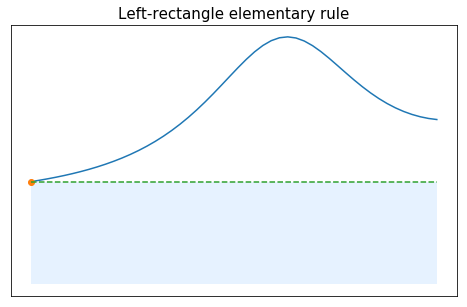
\includegraphics[scale=0.23]{RectL_Elem.png}
        \hspace{16pt}
        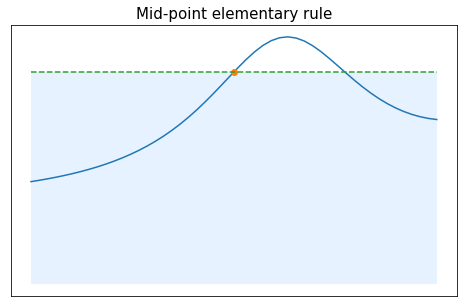
\includegraphics[scale=0.23]{MP_Elem.png}
        \hspace{16pt}
        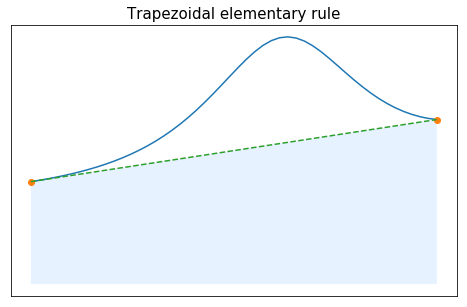
\includegraphics[scale=0.23]{Trap_Elem.png}
        \hspace{16pt}
        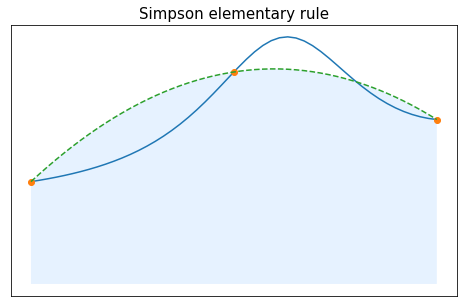
\includegraphics[scale=0.23]{Simpson_Elem.png}

        \hspace{1pt}
        a.Left rectangle rule
        \hspace{30pt} 
        b.Mid-point rule
        \hspace{44pt}
        c.Trapezoidal rule
        \hspace{44pt}
        d.Simpson's rule

        \vspace{10pt}

        We get that that
        
        \begin{table}[H]
            \centering
            \begin{tabular}{|c|c|c|c|}
                \hline
                \rowcolor{gray!30} elementary rule & degree $n$ & symmetry and $n$ even & order of accuracy $n_a$ \\
                \hline
                Left rectangle & $n=0$ & no & $n_a = 0$ \\
                \hline
                \rowcolor{gray!10} Mid-point & $n=0$ & yes & $n_a = 1$ \\
                \hline
                Trapezoidal & $n=1$ & no & $n_a = 1$ \\
                \hline
                \rowcolor{gray!10} Simpson & $n=2$ & yes & $n_a = 3$ \\
                \hline
            \end{tabular}
            % \caption{Your table caption here}
            \label{tab:What}
        \end{table}

        \vspace{10pt}

        \begin{theorem}{Proposition}
            Consider $n+1$ interpolation nodes $x_0<\ldots<x_n$ in $[-1,1]$, and the associated quadrature rule $I^n_{[-1,1]}$ based on Lagrange interpolation (which we already know to be of order at least $n$). If $n$ is even, and the nodes are symmetric with respect to $0$, then the rule is of order at least $n+1$.
        \end{theorem}

        \newpage

        \subsubsection{Clenshaw-Curtis quadrature}

        \begin{definition}{Clenshaw-Curtis quadrature rules}
            The Clenshaw-Curtis quadrature rules are the quadrature rules based on Lagrange interpolation with Chebyshev nodes.
        \end{definition}

        \vspace{10pt}

        \begin{theorem}{Theorem}
            For any integer $n$, the weights $\omega_k$ ($k=0,..,n$) of the Clenshaw-Curtis quadrature rule of degree $n$ are all positive.
        \end{theorem}

        \subsubsection{Gaussian quadrature}

        \vspace{10pt}

        \begin{other}{Legendre orthogonal polynomials}
            There exists a unique family of polynomials $\left(Q_n\right)_{n\geq 0}$ verifying

            $\bullet$ $Q_n$ is of degree $n$,
            
            $\bullet$ $\displaystyle \int_{-1}^1 P(x) Q_n(x) dx = 0$ for any polynomial $P$ of degree at most $n-1$,
            
            $\bullet$ $Q_n(1)=1$.
            
            These polynomials are called the Legendre polynomials. It can be proven that they have $n$ distinct roots in $(-1,1)$.
        \end{other}

        \vspace{10pt}

        \begin{definition}{Gaussian (or Gauss-Legendre) quadrature rule}
            The \textbf{Gaussian (or Gauss-Legendre) quadrature rules} are the quadrature rules based on Lagrange interpolation for which the $n+1$ nodes are the roots of the $n+1$-th Legendre polynomial $Q_{n+1}$.
        \end{definition}

        \vspace{10pt}

        \begin{theorem}{Theorem}
            The Gaussian (or Gauss-Legendre) quadrature rule of degree $n$ (i.e. with $n+1$ nodes) is of order of accuracy $n_a=2n+1$.

            For the Gauss-Legendre quadrature, all the weights $\omega_k$ are positive for all $n$.
        \end{theorem}

        \vspace{10pt}

        \begin{theorem}{Theorem}
            Let $f$ be a continuous function on $[-1,1]$, and $I^n_{[-1,1]}$ be either the Clenshaw-Curtis or the Gauss-Legendre rule of degree $n$. Then
            \begin{align*}
            \lim_{n\to+\infty} I^n_{[-1,1]}(f)  = \int_{-1}^1 f(x) dx .
            \end{align*}
        \end{theorem}

    \subsection{Composite integration}

    \begin{definition}{Composite quadrature rule}
        Consider an interval $[a,b]$, a set of $m+1$ mesh points $(t_j)_{0\leq j\leq m}$ such that $a = t_0 < t_1 < \ldots < t_m = b$, and an integer $n$. A **composite quadrature rule** of degree $n$ associated to the mesh $(t_j)_{0\leq j\leq m}$ is an approximation of $\int_a^b$ of the following form 
        $$
        \int_a^b f(x)dx = \sum_{j=0}^{m-1} \int_{t_j}^{t_{j+1}} f(x)dx  \approx \sum_{j=0}^{m-1} I^n_{[t_j,t_{j+1}]}(f),
        $$
        
        where $I^n_{[t_j,t_{j+1}]}$ is an elementary quadrature rule of degree $n$ on $[t_j,t_{j+1}]$.
        
        We denote by $E_m(f)$ the error
        $$
        E_m(f) = \left\vert \int_a^b f(x)dx - \sum_{j=0}^{m-1} I^n_{[t_j,t_{j+1}]}(f) \right\vert ,
        $$
        associated to such a composite quadrature rule (the error also depends on $n$, on $[a,b]$, and on the mesh, but our focus will be on the behavior of the error when $m$ goes to infinity).
    \end{definition}

    \vspace{10pt}

    \begin{other}{Composite left rectangle method}
        \vspace{4pt}
        \noindent
        For $n=0$, if we use the left rectangle elementary rule on each subinterval we obtain:
        $$
        \int_a^b f(x)dx  \approx \sum_{j=0}^{m-1} I^0_{[t_j,t_{j+1}]}(f) = \sum_{j=0}^{m-1} (t_{j+1}-t_j)\,f(t_j).
        $$
        If we use a uniform mesh, we simply get the following formula for the composite left rectangle method:
        $$
        \int_a^b f(x)dx  \approx \frac{b-a}{m}\sum_{j=0}^{m-1} f(t_j).
        $$
    \end{other}

    \vspace{10pt}

    \begin{other}{Composite mid-point method}
        Still for $n=0$, if we instead use the mid-point elementary rule on each subinterval we obtain:
        
        $$
        \int_a^b f(x)dx  \approx \sum_{j=0}^{m-1} (t_{j+1}-t_j)\,f(t_{j+1/2}),
        $$
        
        which, for a uniform mesh, simplifies into
        
        $$
        \int_a^b f(x)dx  \approx \frac{b-a}{m}\sum_{j=0}^{m-1} f(t_{j+1/2}),
        $$
        
        where $t_{j+1/2} = \frac{1}{2}(t_j+t_{j+1})$ denotes the mid-point of the subinterval $[t_j,t_{j+1}]$.
    \end{other}

    \vspace{10pt}

    \begin{other}{Composite trapezoidal method}
        For $n=1$, the composite quadrature based on the elementary trapezoidal rule gives:

        $$
        \int_a^b f(x)dx  \approx \sum_{j=0}^{m-1} I^0_{[t_j,t_{j+1}]}(f) = \sum_{j=0}^{m-1} \frac{t_{j+1}-t_j}{2}\,(f(t_j)+f(t_{j+1})).
        $$
        
        If we use a uniform mesh, we simply get the following formula for the composite trapezoidal method:
        
        $$
        \int_a^b f(x)dx  \approx \frac{b-a}{m}\sum_{j=0}^{m-1} \frac{f(t_j)+f_(t_{j+1})}{2} = \frac{b-a}{m}\left(\frac{f(t_0)+f(t_{m})}{2} + \sum_{j=1}^{m-1} f(t_j) \right) .
        $$
    \end{other}

    \vspace{10pt}

    \begin{remark}
        Using a logarithmic scale for both the error and $m$, we get lines in the plot, i.e.
        $$
        \ln (E_m(f)) \approx \alpha \ln m + \beta,
        $$
        which suggests that we could have
        $$
        E_m(f) = \frac{C}{m^{-\alpha}}.
        $$
    \end{remark}

    \subsubsection{Error and rate of convergence}

    \begin{theorem}{Convergence of composite quadrature rules}
        Consider an interval $[a,b]$, a set of $m+1$ mesh points $(t_j)_{0\leq j\leq m}$ such that $a = t_0 < t_1 < \ldots < t_m = b$, an integer $n$, and a composite quadrature rule of the form 
        
        $$
        \int_a^b f(x)dx = \sum_{j=0}^{m-1} \int_{t_j}^{t_{j+1}} f(x)dx  \approx \sum_{j=0}^{m-1} I^n_{[t_j,t_{j+1}]}(f).
        $$
        
        If the elementary quadrature rule used on each subinterval $[t_j,t_{j+1}]$ is of order of accuracy at least $n_a$, and $f\in{\cal C}^{n_a+1}([a,b])$, then there exists a constant $C$ (independent of $m$), such that the error is bounded as follows:
        
        $$
        E_m(f) \leq C \sup_{x\in [a,b]} \left\vert \,f^{(n_a+1)}(x)\,\right\vert (b-a) \, h^{n_a+1},
        $$
        
        where we recall that 
        
        $$h = \max_{j=0,\ldots,m-1} \left\vert t_{j+1} - t_j \right\vert.$$
    \end{theorem}

    % \begin{remark}
    %     $\bullet$ In the case of a uniform mesh, where $h=(b-a)/m$, we get 
    %     $$
    %     E_m(f) \leq \frac{C \sup_{x\in [a,b]} \left\vert f^{(n_a+1)}(x)\right\vert (b-a)^{n_a+1}}{m^{n_a+1}}.
    %     $$
    %     $\bullet$ This is a typical case of *sublinear* convergence, as introduced in the first chapter, at least for the error bound $\beta_m = \frac{C \sup_{x\in [a,b]} \left\vert f^{(n_a+1)}(x)\right\vert (b-a)^{n_a+1}}{m^{n_a+1}}$, since 
    %     $$
    %     \frac{\beta_{m+1}}{\beta_m} \underset{m\to\infty}{\longrightarrow} 1.
    %     $$
    % \end{remark}
\end{document}
